\chapter{Introduction}
\label{cha:introduction}





\section{Idea of Cluster-wise Encoding}
\label{sec:clusterSearch}

The goal of this task is to optimize the encoding of state machines within an FPGA.\\
Usually state machines on FPGAs are one-hot encoded to minimize the logic necessary for the transitions. However, if a state machine is small enough to be placed within one lookup-table it can be binary encoded. Generally this encoding is preferable since it is more compact, but also fast.

To optimize the encoding of a state machine we try to sort as many states as possible into clusters that represent binary encoded sub- state machines, which can be implemented in one lookup-table.\\
Mathematically speaking we try to minimize the number of clusters that can fulfill constraints that allow them to be mapped within one lookup-table.\\
Any cluster that can not fulfill this equation or constrains only one state has to be one-hot encoded.
%the following equation:

%$ N\_max\ > N = \#Incoming\_Inter\_Cluster\_Transitions + ld(\#States) + \#Input\_Bits\_That\_Care + 1 $

%Where $ \#Incoming\_Inter\_Cluster\_Transitions $ specifies the number of transitions that origin in other valid clusters and target this cluster. \\
%$ld(\#States)$ is the logarithmus dualis of the number of states contained in the cluster.\\
%$ \#Input\_Bits\_That\_Care $ contains the number of bits that are minimally needed to represent the %input of the transitions within the cluster. For example the number for the transitions with inputs "1--0" and "--1-" would be 3.

\subsubsection{Available LUT Inputs}
\label{subsubsec:LUTInputs}
Each cluster must fit into exactly one slice/lookup table. All necessary inputs and state transition signals must be fed into this LUT. \\
The following equation describes the input of the LUT and the constraints that each cluster must fulfill:

\begin{center}
\begin{eqnarray}
1\vspace{1cm} \label{m1}+\\
log_2(n_{statesInCluster}) \label{m2}+ \\
n_{ExternalInputsThatCare} \label{m3}+ \\
n_{incomingInterClusterTransitions} \label{m4}+ \\
= N \label{m5}\\
<= N_{LUT\_inputs} \label{m6}\
\end{eqnarray}
\end{center}

Equation (\ref{m1}) describes the bit that is necessary to check if the cluster itself is active.\\
The states inside the cluster are encoded binarily, therefore $ld(\text{number of states})$ bits are needed to represent the states (\ref{m2}). \\
It is alse necessary to consider the inputs of the transistions. Only input bits that are not always in the "don't care" state must be considered. Therefore equation (\ref{m3}) describes the number of bits that are minimally necessary to describe an input. \\
Incoming transitions from other clusters also have to be taken into account. Equation (\ref{m4}) describes them with one bit for each transition. \\

It is necessary to always satisfy all these conditions. Therefore, the value $N_{LUT\_inputs}$ or $N\_max$ (\ref{m6}) represents the number of inputs the LUT has, while the value $N$ (\ref{m5}) represents the number of inputs that are already used.
Figure \ref{img:slice7} shows an example how a binary encoded state machine cluster might be implement in an LUT with 7 inputs.


\begin{figure}
	\centering
	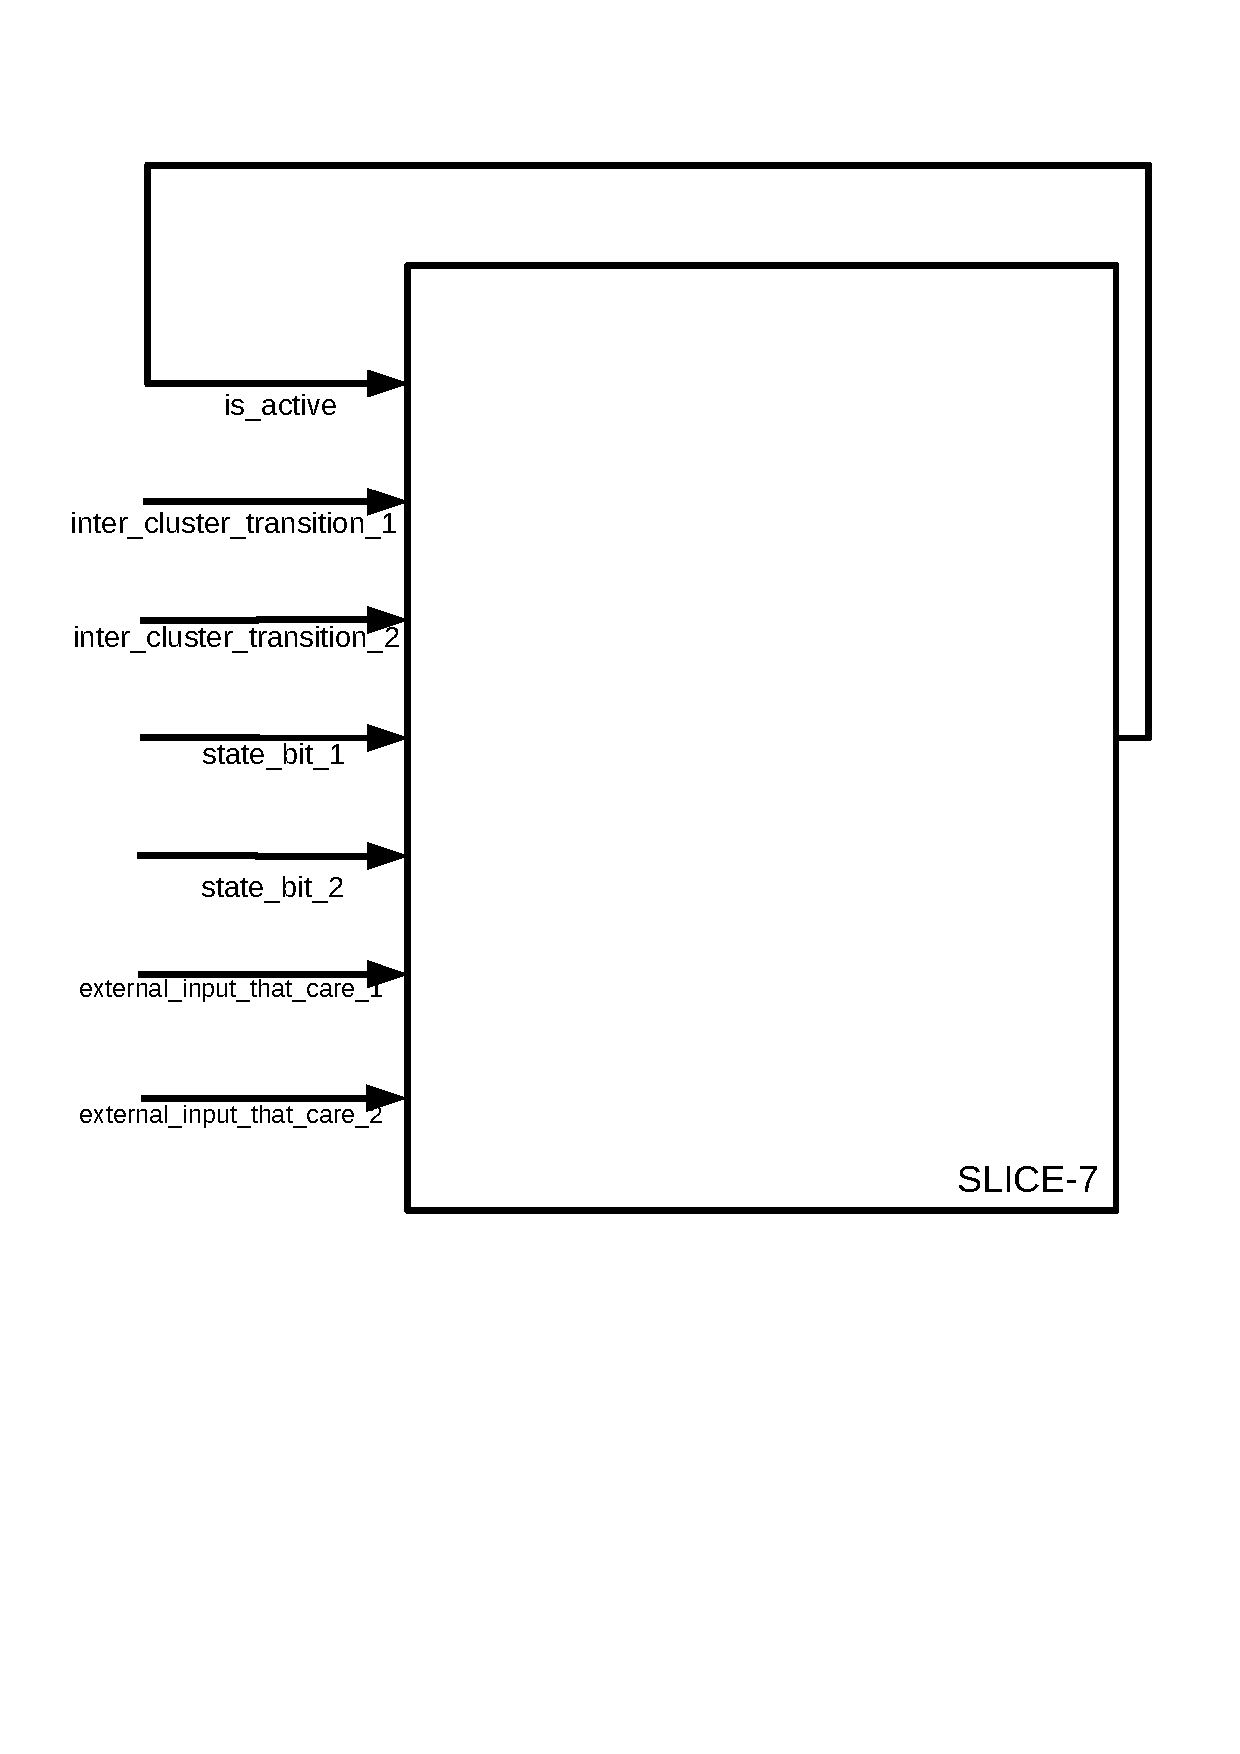
\includegraphics[scale=0.65, trim=400 250 400 97] {images/slice7.pdf}
	\caption{A binary encoded state machine consisting of one LUT with 7 inputs.}
	\label{img:slice7}
\end{figure}




\subsubsection{Algorithm}
\label{subsubsec:algo}

The clustering problem is of combinatorial complexity. This is especially important for large state machines.
Due to this fact no exact solution can be found in polynomial time. A heuristically approach is necessary. \\

Figure \ref{img:state_chart} shows one possible clustering. Red circles represent clusters that can be converted into a binary encoded state machine and yellow circles those that should be one-hot encoded.
All yellow clusters either have an $N$ higher than 6 or only one state. \\

\begin{figure}[h]
	\centering
	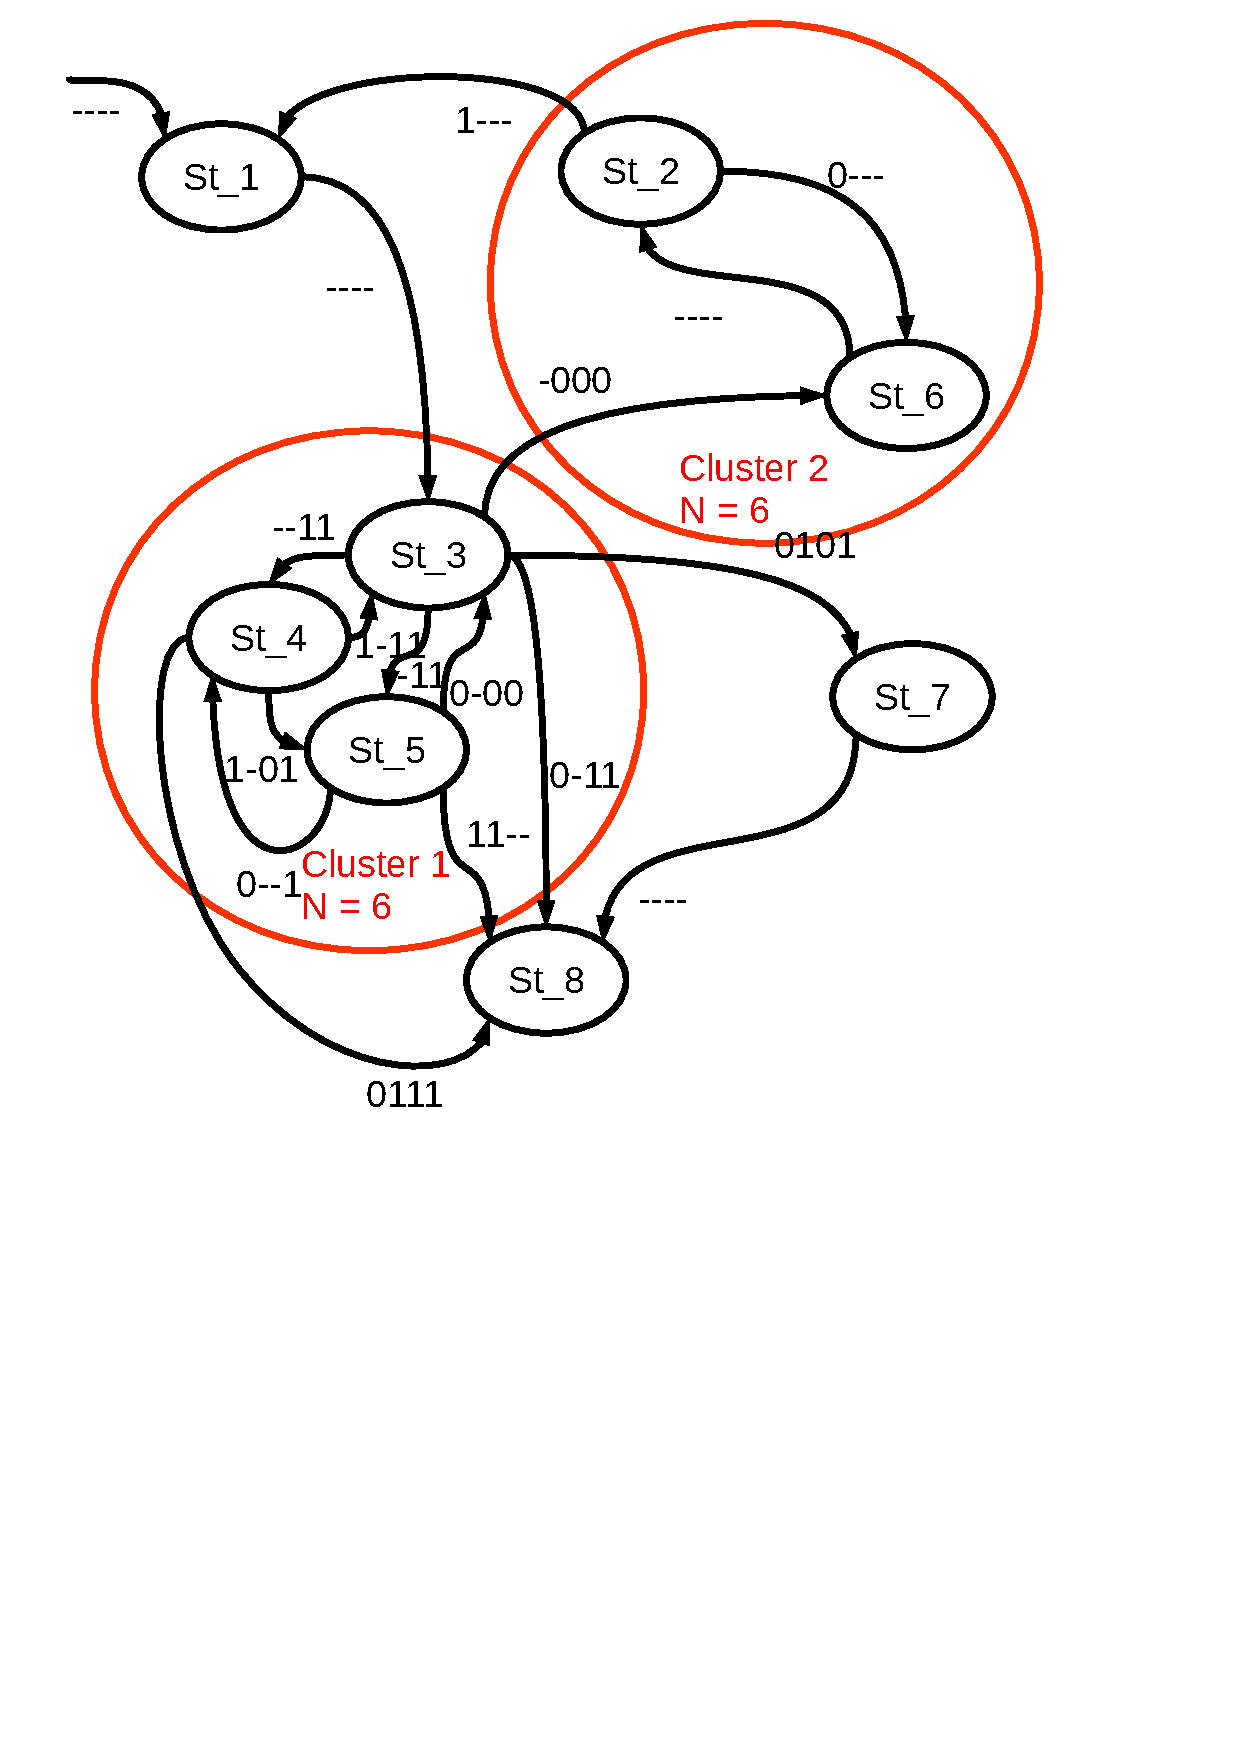
\includegraphics[scale=0.65, trim=400 250 400 0] {images/state_chart.pdf}
	\caption{An example clustering of a small state machine. Red cycles are binary encoded clusters, yellow circles are one-hot encoded.}
	\label{img:state_chart}
\end{figure}

In order to sort the different states into clusters we pursued multiple approaches.
In our first approach, we sort all states into separate clusters and attempt to combine them if possible. \\
This results in a generally bad solution due to the fact that a cluster usually cannot be expanded by just one state. This behavior is a result of the $ incomingInterClusterTransitions $ constraint. \\
While a cluster might be expandable if multiple states (which reference each other) are sorted into the cluster, one state will usually not allow that expansion. \\
In other words, expanding the cluster state by state will result in a solution that only yields a local maximum.\\
This finding leads to a second approach. The second algorithm attempts to create clusters out of states who stand in relationship which each other. To do so the algorithm takes each available cluster once and determines the predecessors of that cluster by following the outgoing transitions. \\
These predecessors are now ordered by the number of different ingoing transitions they have. After the ordering the algorithm tries to merge the clusters. In case that merging violates the constrains the state with the lowest order is thrown away. \\
Due to the fact that this algorithm strongly depends on states that have a lot of corresponding states, this algorithm tends to work bad on the most benchmarks. Therefore, it became clear that an algorithm that works without observation or model based approaches is necessary. \\

For the final approach we apply the simulated annealing technique introduced during the lecture. This algorithm is chosen because of its well-known, problem-independent effectiveness. The task hence reduces to finding a suitable fitness function and mutation scheme.\\
Due to the timed scope of this project no further fine-tuning of the parameters, like starting and end temperature, could be included. \\
Both fitness function and the mutation scheme are described in the next chapter.\\



\chapter{Simulated Annealing}
\label{cha:SimulateAnnealing}

\subsubsection{Simulated Annealing Algorithm}
\label{subsubsec:SAAlgorithm}

We use the simulated annealing algorithm introduced in the lecture. Due to the timed scope of the project we have not optimized the algorithm in terms of its parameters. In the following, the utilized values are presented.

\begin{itemize}
\item[\textbf{Starting temperature}]\hfill \\
As starting temperature, the standard deviation of N random solutions' fitness difference, multiplied with 20, has been assumed, where N equals the number of states to encode.
\item[\textbf{End temperature}]\hfill \\
Since there was no experience regarding the runtime of the algorithm for the clustering problem on the benchmarks' state graphs, we started with an end temperature of 0.01. This value worked well and has therefore not been altered.
\item[\textbf{Inner number}]\hfill \\
For the sake of short runtime, the inner number has been chosen as 1.0.
\item[\textbf{Temperature update}]\hfill \\
After each outer loop iteration, the temperature is updated according to the current acceptance rate. The multiplicator $\gamma$ as function oftheacceptance rate $\alpha$ is shown below.

\begin{tabbing}
\hspace{4cm}\=\hspace{4cm}\=\hspace{4cm}\=\kill
 \alpha>=0.96  \>\0.96>=\alpha>0.8 \>0.8>=\alpha>0.15  \> 0.15>=\alpha \\ 
 \gamma=0.5 \>  \gamma=0.9 \>  \gamma=0.95 \> \gamma=0.8
\end{tabbing} 
\end{itemize}


With the parameter values shown above, the runtime is in the range of seconds. This behaviour originates in the small problem size compared to typical problems where Simulated Annealing is applied. Considering this, there was no need to otimize the parameter set towards a better runtime.


\subsubsection{Fitness Function}
\label{subsubsec:FitnessFunction}

We try to minimize the number of binary encoded clusters. Therefore the fitness function is declared as the difference between the number of states and the number of current clusters. In mathematical terms: 
\begin{equation}
\text{fitness(solution)} = \sum{\text{states}} - \sum{\text{clusters}}
\end{equation}

It is necessary that we do not break the equation  $N\_max$ (\ref{m6}) for each cluster. Therefore, the fitness of a solution is 0 if $ N $ (\ref{m5}) is greater $N\_max$.

\subsubsection{Mutation}
\label{subsubsec:Mutation}

In order to find a good solution it is necessary to mutate the current cluster structure by interchanging a variable number of states between the clusters. \\
Each mutation operation extracts a random state from its cluster and assignes it to another random cluster. Clusters that lose all their states are deleted. \\
In order to surpass the local minima problem it is possible that one cluster is assigned multiple states.\\
If multiple mutations are performed on one clustering, there is a probability of maximal 25\% that the same cluster is chosen again. Each time the cluster is chosen again this probability is lowered by 5\,\%.


\chapter{Evaluation}
\label{cha:Evaluation}

This chapter evaluates the quality of the cluster-based state encoding.
\subsubsection{BLIF Format as Output}
\label{subsubsec:BLIFOutput}

NEU SCHREIBEN WEIL IST NICHT
Initial we choose BLIF as our format of choice to encode the different state machines. While the encoding process itself is functional the ABC parsers additionaly needs XYZ.
Due to time constrains we were not able to parse our state machines into the ABC parser. Instead we choose to estimate the number of LUT and FF based on the structure of the FSM.

\subsubsection{Ideal Results}
\label{subsubsec:IResults}

The following diagram shows the number of lookup-tables and Flip Flops that is minimal needed to encode the states machines. This number is based on the ideal model that one lookup-table is needed for one binary cluster or one one-hot encoded state. This model excludes all additional lookup-tables needed for transition purposes.


\subsubsection{Practical Results}
\label{subsubsec:PResults}

In order to actually implement the state machines additional lookup-tables to represent the transtion logic are needed. 
Due to the fact that XYZ we need additional XXX.
The following


\subsubsection{Conclusion}
\label{subsubsec:Conclusion}

While the numbers of our initial ideal model showed promises .
While did not had the time to validated we believe that We hope that we can validate our work with BILF within the next weeks but 



The BLIF format for finite state machines as described in \cite{blif} has some advantages which qualify it over a HDL representation as output format. Among these are the the good parseability, which is especially useful in small projects, and its independence of a specific platform.
Additionally, the input files describing state machines in the scope of this project are .kiss filesm which are a subspecification of the BLIF format. Therefore, only the circuit mapping has to be written to the output file, and no conversion from BLIF to a HDL description of the functional behaviour has to be pursued. The .kiss format does not allow a more detailed circuit description than the mapping of latches. This must be done in a detailed .blif file. In our case, this disadvantage could be neglected, so that BLIF was the output format of choice.

\subsubsection{Achievements}
\label{subsubsec:Achievements}

The presented method is capable of parsing .kiss2 files describing the behaviour of finite state machines, finding clusters of the included states
according to an optimization towards their mapping to FPGA lookup tables and assigning codes to these found clusters. The results are written back into a .blif file containing the logical description and the codes for each cluster and state. Clusters are determined so that the logic associated with each of them fits into one lookup table. In the scope of this project, some parameter restrictions had to be assumed. The amount of inputs for available LUTs was assumed as 8, which is a possible input count in modern FPGA series. For thenumber of external inputs of the finite state machine, the soft limit of 4 is used. This value has been chosen so that the limitations for one cluster can be ensured; nevertheless, larger input counts may work depending on the amount of significant (i.e. non-don't-care) bits in the input vectors.
